% !TeX encoding = UTF-8
\documentclass[aspectratio=169]{beamer}
\useoutertheme[progressbar=frametitle]{metropolis}
\useinnertheme{metropolis}
\definecolor{nabgray}{rgb}{0.6,0.59,0.61}
\usecolortheme[named=nabgray]{structure}

\usepackage{tikz}
\usepackage[utf8]{inputenc}
\usepackage[spanish]{babel}
\usepackage{fontspec}
\setmonofont{JetBrains Mono}
\setmainfont{Roboto}
\setsansfont{Roboto}

\usepackage{smartdiagram}
\usepackage{qtree}
\usepackage{verbatim}
\usepackage{svg}
\usepackage{graphicx}
\usepackage{color}

\definecolor{lightgray}{rgb}{0.95, 0.95, 0.95}
\definecolor{darkgray}{rgb}{0.4, 0.4, 0.4}
%\definecolor{purple}{rgb}{0.65, 0.12, 0.82}
\definecolor{editorGray}{rgb}{0.95, 0.95, 0.95}
\definecolor{editorOcher}{rgb}{1, 0.5, 0} % #FF7F00 -> rgb(239, 169, 0)
\definecolor{editorGreen}{rgb}{0, 0.5, 0} % #007C00 -> rgb(0, 124, 0)
\definecolor{orange}{rgb}{1,0.45,0.13}
\definecolor{olive}{rgb}{0.17,0.59,0.20}
\definecolor{brown}{rgb}{0.69,0.31,0.31}
\definecolor{purple}{rgb}{0.38,0.18,0.81}
\definecolor{lightblue}{rgb}{0.1,0.57,0.7}
\definecolor{lightred}{rgb}{1,0.4,0.5}
\usepackage{upquote}
\usepackage{listings}
\lstset{language=java,
	basicstyle=\footnotesize\ttfamily,
	keywordstyle=\footnotesize\color{blue}\ttfamily,
	escapeinside={<@}{@>}
}
\lstdefinelanguage{Kotlin}{
	comment=[l]{//},
	commentstyle={\color{gray}\ttfamily},
	emph={delegate, filter, first, firstOrNull, forEach, lazy, map, mapNotNull, println, return@},
	emphstyle={\color{purple}},
	identifierstyle=\color{black},
	keywords={abstract, actual, as, as?, break, by, class, companion, continue, data, do, dynamic, else, enum, expect, false, final, for, fun, get, if, import, in, interface, internal, is, null, object, override, package, private, public, return, set, super, suspend, this, throw, true, try, typealias, val, var, vararg, when, where, while},
	keywordstyle={\color{lightblue}\bfseries},
	morecomment=[s]{/*}{*/},
	morestring=[b]",
	morestring=[s]{"""*}{*"""},
	ndkeywords={@Inject, @Deprecated, @JvmField, @JvmName, @JvmOverloads, @JvmStatic, @JvmSynthetic, Array, Byte, Double, Float, Int, Integer, Iterable, Long, Runnable, Short, String},
	ndkeywordstyle={\color{orange}\bfseries},
	sensitive=true,
	stringstyle={\color{olive}\ttfamily},
}

\usebackgroundtemplate%
{%
	
\includegraphics[width=\paperwidth]{Images/Contenido}%
}


\title{Compilación nativa con Kotlin y GraalVM}
\author{Víctor Orozco}
\institute{Nabenik}
\date{\today}

\begin{document}





{
    \usebackgroundtemplate{
\includegraphics[width=\paperwidth]{Images/portada}}
    \setbeamercolor{frametitle}{fg=red}
    \usebeamercolor[fg]{normal text}
    \frame{\titlepage}
}


\begin{frame}{Ecosistema Kotlin}
\begin{figure}
	\centering
	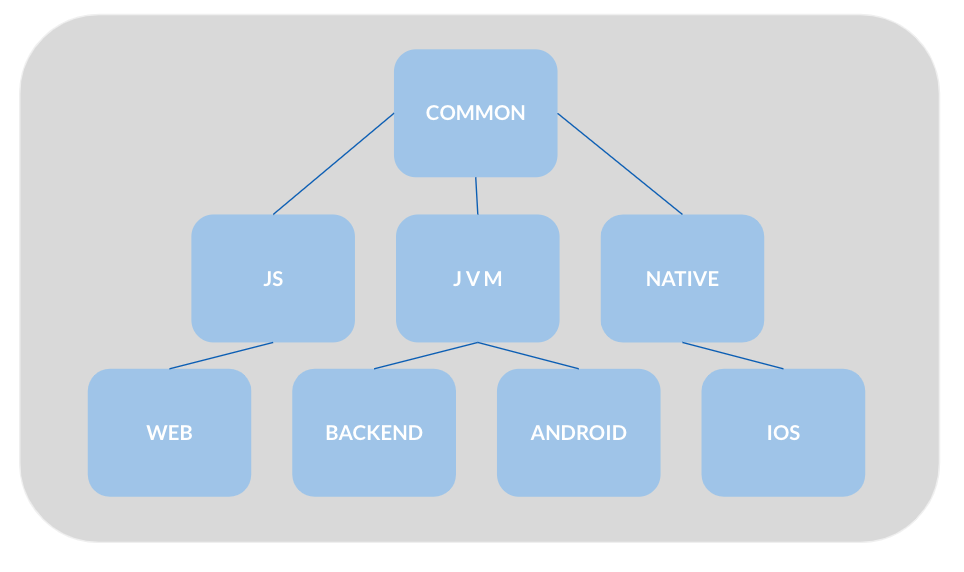
\includegraphics[width=0.8\linewidth]{Images/KotlinNative.png}
	\label{fig:kotlin}
\end{figure}
\end{frame}


\begin{frame}{Kotlin Native}
	\begin{columns}[T] % contents are top vertically aligned

		\begin{column}[T]{6cm} % alternative top-align that's better for graphics
			Kotlin Native
		\begin{enumerate}
		\item Código Kotlin + Kotlin stdlib + Bibliotecas "Kotlin puro"
		\item Bytecode LLVM
		\item Bibliotecas del sistema -e.g. Cocoa -
		\end{enumerate}
		\end{column}
		\begin{column}[T]{6cm} % each column can also be its own environment
        Kotlin GraalVM Native
        \begin{enumerate}
        \item Código Kotlin + Kotlin stdlib + \textbf{Bibliotecas JVM}
        \item Aplicaciones ELF / Mach-O con GCC
        \item LLVM backend
        \item SubstrateVM
        \end{enumerate}

		\end{column}
	\end{columns}
\end{frame}


\begin{frame}{GraalVM}
¿GraalVM?
	\begin{itemize}
		\item Maquina virtual poliglota de Oracle Labs
		\item JVM, Truffle, LLVM
        \item Escrita en Java
        \item Open Source y Enterprise Edition
	\end{itemize}
\end{frame}


\begin{frame}{}
\begin{figure}
	\centering
	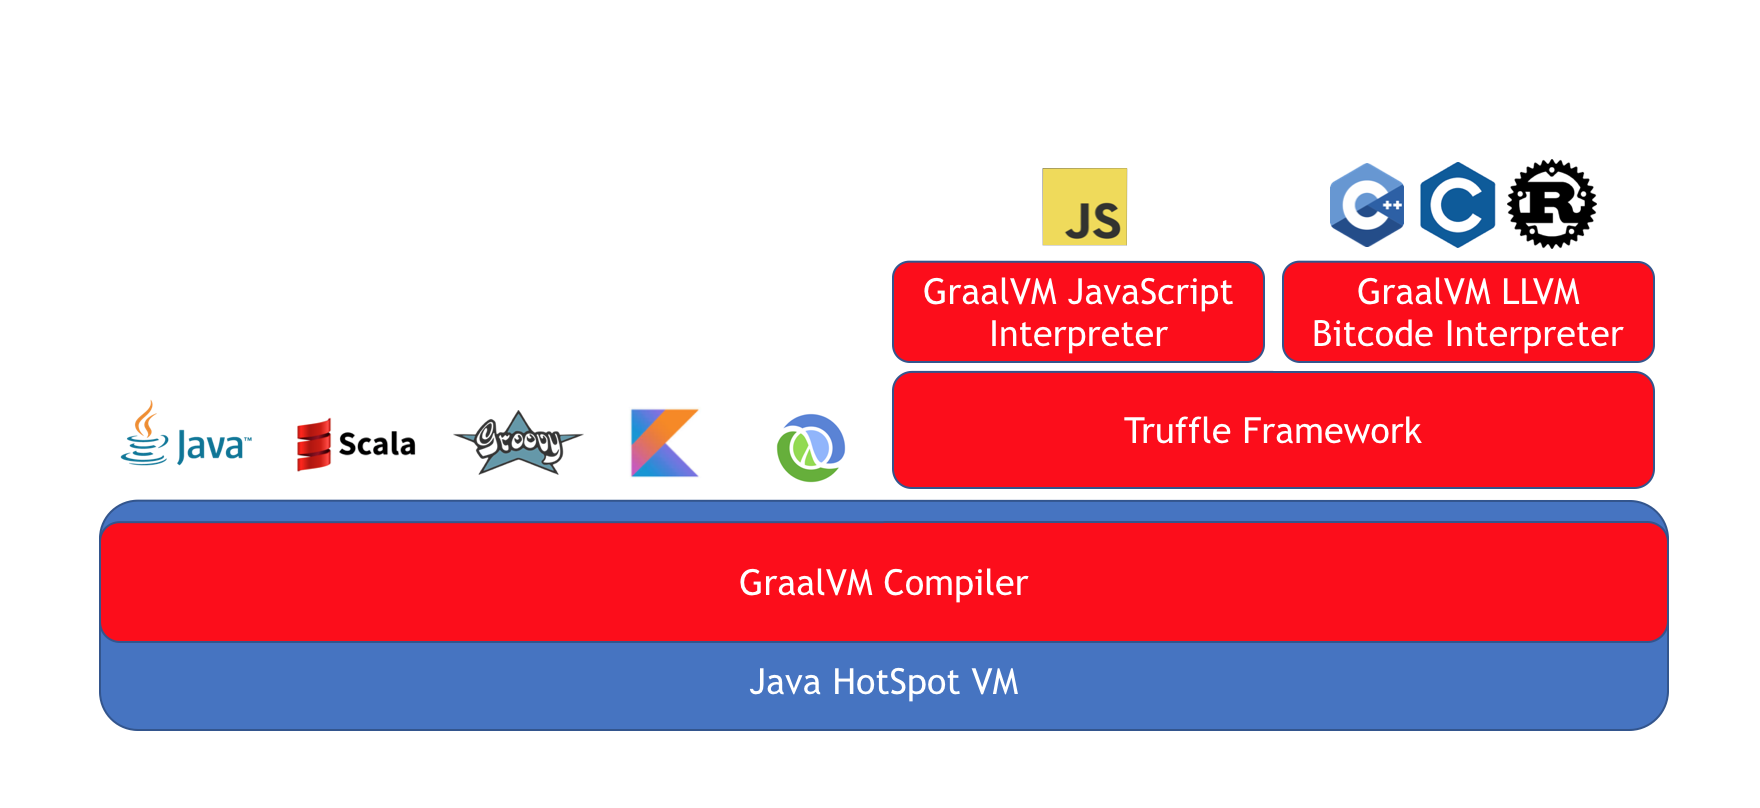
\includegraphics[width=\linewidth]{Images/graalvm}
	\caption{GraalVM Overview}
	\label{fig:graalvm}
\end{figure}

\end{frame}

\begin{frame}{GraalVM}

	\begin{columns}[T] % contents are top vertically aligned

		\begin{column}[T]{4cm} % alternative top-align that's better for graphics
			Hechos importantes
		\begin{enumerate}
			\item TCK'd JDK
			\item Compilador JIT
			\item \textbf{Java Native Image}
			\item Polyglot VM
		\end{enumerate}
		\end{column}
		\begin{column}[T]{6cm} % each column can also be its own environment
			\begin{figure}
				\centering
				
\includegraphics[width=\linewidth]{Images/graalvmlogo}

			\end{figure}

		\end{column}
	\end{columns}


\end{frame}

{
	\usebackgroundtemplate{
\includegraphics[width=\paperwidth]{Images/separador}}
	\setbeamercolor{normal text}{fg=white}
	\setbeamercolor{frametitle}{fg=red}
	\usebeamercolor[fg]{normal text}
	\section{Imagenes nativas}
}



\begin{frame}{Java Virtual Machine}

	\begin{itemize}
		\item Thread scheduling, gestión de memoria
		\item JVM JIT (C2) tem 25 anos
		\item Peak performance
		\item Hotspots
	\end{itemize}

\end{frame}


\begin{frame}{GraalVM Native}
	\begin{figure}
		\centering
		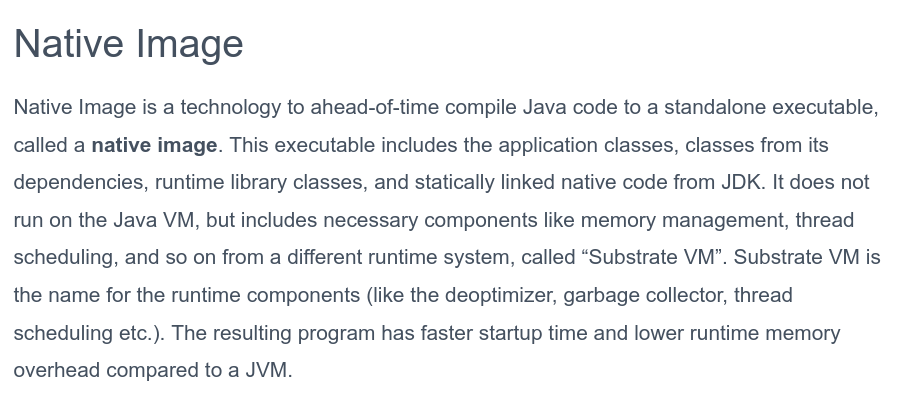
\includegraphics[width=\linewidth]{Images/nativeimagedefinition.png}
	\end{figure}
{\tiny https://www.graalvm.org/reference-manual/native-image/}
\end{frame}


\begin{frame}{GraalVM Native}

	\begin{exampleblock}{GraalVM Native}
	GraalVM Native es una tecnología para \textbf{compilación AOT de bytecode}. Permite crear un ejecutable \textbf{self-contained} con \textbf{static linking} de clases, bibliotecas y módulos de la JVM.
	\end{exampleblock}

\end{frame}




\begin{frame}{AOT en el mundo de la JVM}
	\begin{itemize}
		\item ExcelsiorJET
		\item GNU Compiler for Java
		\item ART (Android)
		\item \textbf{IBM OpenJ9}
	\end{itemize}

\end{frame}



\begin{frame}{GraalVM Native}
	\begin{figure}
		\centering
		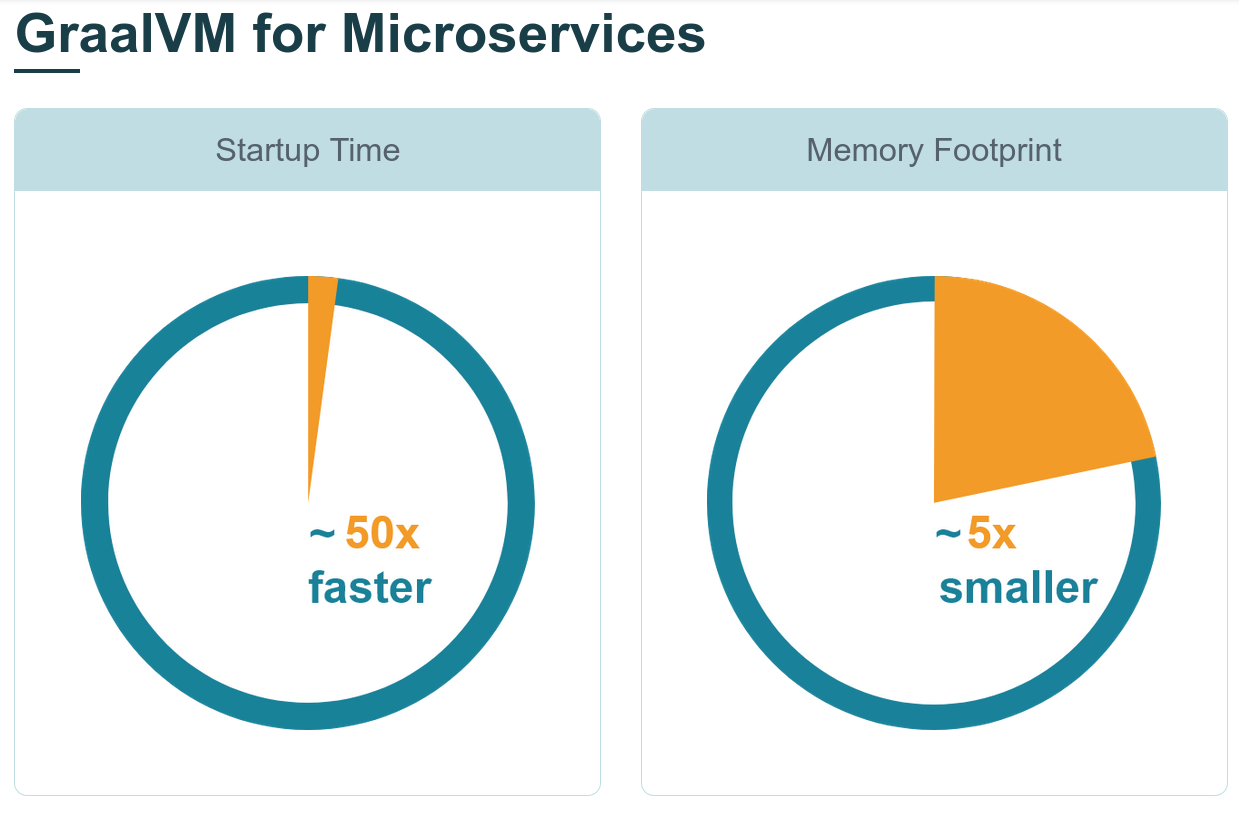
\includegraphics[width=0.7\linewidth]{Images/ventajasnative}
	\end{figure}
\end{frame}


\begin{frame}{GraalVM Native}
	\begin{itemize}
		\item \textbf{CLI}
		\item Apps desktop
    		\item Serverless
		\item \textbf{Microservicios}
        \item Kubernetes operators
	\end{itemize}

\end{frame}

\begin{frame}[fragile]{GraalVM Native}
picocli (Anotaciones)
\begin{lstlisting}[language=Kotlin]
@CommandLine.Command(name = "kobsidian-backup",
mixinStandardHelpOptions = true,
version = ["kobsidian-backup 1.0.10"],
description = ["Creates backups from Postgres and uploads these to Dropbox"])
class BackupOptions{


    @CommandLine.Option(names = ["-d", "--database"],
        paramLabel = "DATABASE NAME",
        description = ["Database target for backup actions"]
    )
    var databaseName: String?
\end{lstlisting}
\end{frame}

\begin{frame}[fragile]{GraalVM Native}
clikt (Kotlin DSL)
\begin{lstlisting}[language=Kotlin]
class Hello : CliktCommand() {
    val count: Int by option(help="Number of greetings").int().default(1)
    val name: String by option(help="The person to greet").prompt("Your name")

    override fun run() {
        repeat(count) {
            echo("Hello $name!")
        }
    }
}
\end{lstlisting}
\end{frame}

\begin{frame}{Kobsidian Backups}
	\begin{figure}
		\centering
		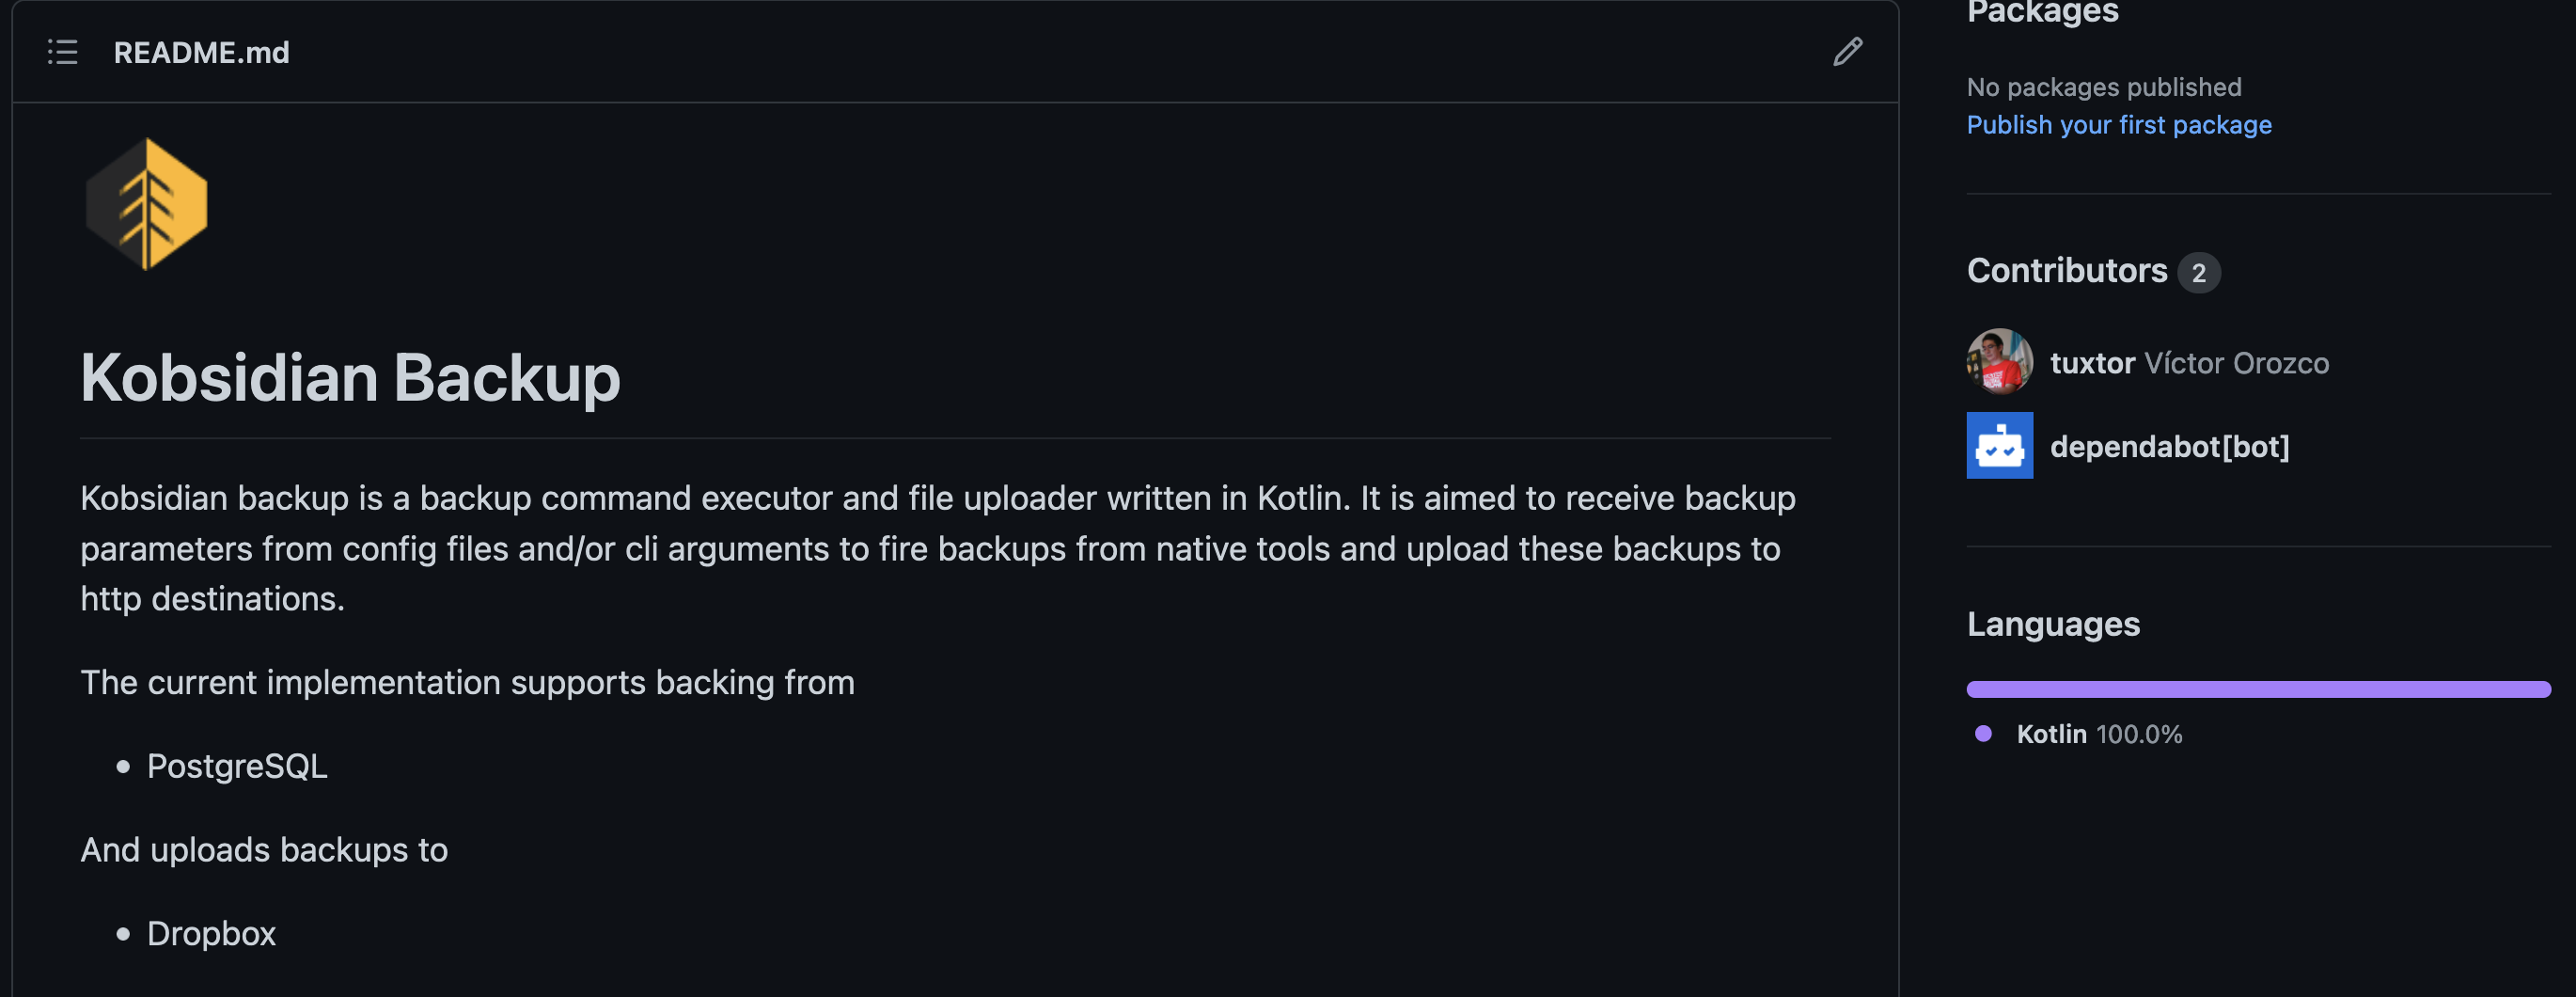
\includegraphics[width=\linewidth]{Images/kobsidian.png}
	\end{figure}
\end{frame}


\begin{frame}{Demo}
	\begin{enumerate}
		\item Maven Quickstart (Java)
		\item Kotlin stdlib
        \item PicoCLI
        \item GraalVM Native
	\end{enumerate}
\end{frame}



{
	\usebackgroundtemplate{
\includegraphics[width=\paperwidth]{Images/separador}}
	\setbeamercolor{normal text}{fg=white}
	\setbeamercolor{frametitle}{fg=red}
	\usebeamercolor[fg]{normal text}
	\section{Consideraciones finales}
}


\begin{frame}{Consideraciones finales}

	\begin{columns}[T] % contents are top vertically aligned

		\begin{column}[T]{4cm} % alternative top-align that's better for graphics
			\begin{exampleblock}{Ventajas}
				\begin{itemize}
					\item Compilación AOT
					\item Consumo de memoria
					\item Tiempo de inicio
					\item CLI, Desktop, Serverless, K8S
				\end{itemize}
			\end{exampleblock}
		\end{column}
		\begin{column}[T]{6cm} % each column can also be its own environment
			\begin{alertblock}{Desventajas}
				\begin{itemize}
					\item Desempeño inferior en el largo plazo
					\item Reflection, dynamic proxies, invoke, bytecode generation
					\item Muchos frameworks jamas seran Cloud Native
					\item Un buen servidor CI/CD
				\end{itemize}
			\end{alertblock}
		\end{column}
	\end{columns}
\end{frame}


\begin{frame}{}
	\begin{figure}
		\centering
		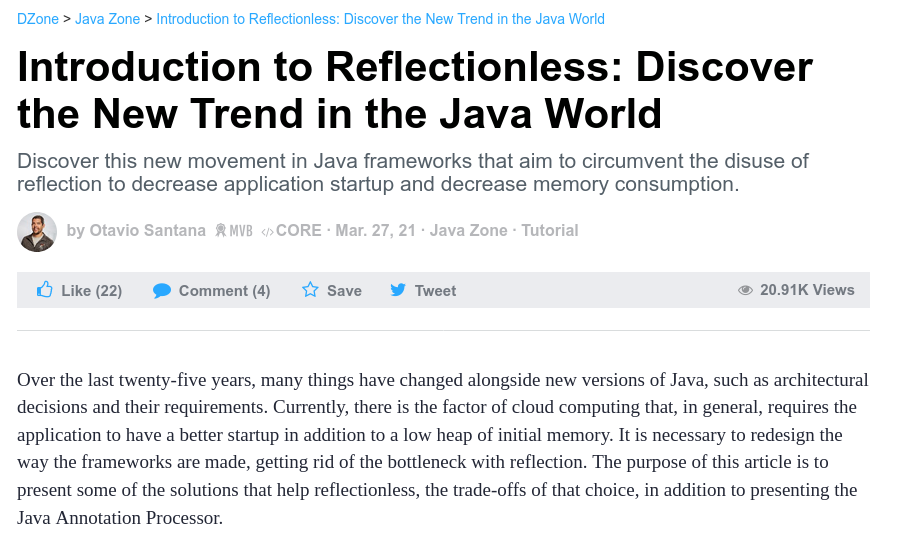
\includegraphics[width=0.8\linewidth]{Images/otavio}
	\end{figure}
{\tiny https://dzone.com/articles/introduction-to-reflectionless-know-what-the-new-t}
\end{frame}

\begin{frame}{Víctor Orozco}
    \begin{columns}[T] % contents are top vertically aligned

        \begin{column}[T]{4cm} % alternative top-align that's better for graphics
            \begin{figure}
                \centering
                
\includegraphics[width=\linewidth]{Images/logos}
            \end{figure}
        \end{column}
        \begin{column}[T]{6cm} % each column can also be its own environment
            \begin{itemize}
                \item vorozco@nabenik.com
                \item \href{https://twitter.com/tuxtor}{@tuxtor}
                \item \href{http://vorozco.com}{http://vorozco.com}
                \item \href{http://tuxtor.shekalug.org}{http://tuxtor.shekalug.org}
            \end{itemize}
            \begin{center}
                
\includegraphics[width=0.1\linewidth]{Images/cclogo}
                \\
                This work is licensed under Creative Commons Attribution-NonCommercial-ShareAlike 3.0 Guatemala (CC BY-NC-SA 3.0 GT).
            \end{center}
        \end{column}
    \end{columns}
\end{frame}



\end{document}
